\section{Introduction} \label{sec:intro}

% (1 Page)
% Present Tense

\begin{comment}
    - Massive Amount of Data
    - Astronomers overloaded
    - Step by step task of astronomer
    - Need to automatize process
    - Focus of solution
    - Final objective of solution
    - Automatic Proposed Algorithm
    - Algorithm Operation Detail
    - Strengths and limitations
    - Conclusions
    - List of Content
\end{comment}

Modern astronomical observatories have brought increasing amounts of data over the last few years.
Radio-telescopes's sensors have improved with higher resolution and wider wavelength ranges sensors.
Instruments like the Atacama Pathfinder Experiment (APEX) \citep{gusten_apex},
the Sub-millimeter Array (SMA) \citep{ho_submillimeter_2004},
Heterodyne Instrument for the Far Infrared (HIFI) \citep{de_graauw_herschel},
Stratospheric Observatory For Infrared Astronomy (SOFIA) \citep{becklin_stratospheric_2005}
and the Atacama Large Millimeter Array (ALMA) \cite{},
will provide higher resolution and details from sub-millimeter regions that will make this region very attractive for spectroscopy
\citep{schilke_line_2001, muller_cologne_2005, schilke_analysis_2011}.

% Astronomers overloaded
% Given this  growing amount of high spectral resolution data, any non-automatic analysis would be an effort beyond human capacity.
With the imminent data growth together with higher sensitivity and resolution will allow an analysis at a much more detailed level.
This makes it impractical for astronomers to process and analyze all the data in a traditional, pedestrian way \citep{schilke_analysis_2011, skoda_spectroscopic_2014}.
% Step by step task of astronomer
% Currently, identifying emission lines involves to estimate their belonging to certain isotopes through the analysis of the isotope lines characteristics.
The traditional spectra analysis to identify emission lines involves the search of similar lines characteristics, such as wavelength, intensity and the presence or absence of other observed lines for each possible isotope \citep{sharpee_introducing_2003}.
Making use of their intuition and experience, astronomers estimate each possible presence of peaks to relate them to known molecules of interest \citep{schilke_analysis_2011}.
% Need to automatize process
% This is a time consuming process for astronomers and automating of this task becomes necessary.
%Tenías esta referencia ( \citep{sharpee_introducing_2003, tonegawa_field:_2015, schilke_analysis_2011} ) después del párrafo siguiente, ¿porqué?
This process is very time-consuming, consequently, it would be of a great help to have an automatic tool that contributes to the analysis.
Several approaches to this problem have been proposed, including models that simulate molecular spectra \citep{schilke_line_2001, comito_molecular_2005, maret_weeds:_2010, caux_cassis_2011, vastel_cassis_2015},  models that fit synthetic spectra with observed ones \citep{pequignot_deep_1996, walsh_deep_2003}, and heuristic analysis of simultaneous presence of lines \citep{sharpee_introducing_2003}.

 % 2. Need (what you want =/= what you have)
% Focus of this work
% An automatic line-classification algorithm would dramatically reduce human efforts to analyse spectral data.
In this work, we propose an automatic line-classification algorithm to support astronomers in spectral data analysis.
Our approach is by no means an exhaustive solution, but a way to reduce scientists's efforts in pre-classification of lines.

 % 3. Task (what I/we did, given this need)
% Automatic Proposed Algorithm
% For this purpose, we propose an algorithm that uses a modeling with sparse representation to classify emission lines.
The proposed algorithm does not rely on any physical model about spectra, it just learns a suitable spectra representation from data.
This representation allows the model to find line-detection patterns that constitute the key of automatic classification.

% Detailing Algorithm Operation
% The algorithm models the spectra to predict the presence of emission lines and their belonging to different isotope transition states.
We work with three-dimensional velocity data cubes that follow ALMA data structure, i.e., intensity as a function of both position and velocity, or it's equivalent frequency, as shown in figure \ref{fig:data_cube} \citep{eguchi_superluminal_2013}. The algorithm takes as input the observed spectra from a data cube, and the output corresponds to a list of candidate emission lines present along the spectra.

    % 4. Object (what the document covers)
%[KP: Arreglar esta parte, estructuras paralelas]
The algorithm has two general steps: i) detection of a list of candidate frequency ranges; ii) confirm the candidate frequency ranges that belong to known isotopes. Step i) uses an heuristic that compares intensity differences along the spectra.
Each consecutive pair of frequencies is evaluated by looking for intensity differences greater than a threshold parameter.
This threshold parameter is given by the 3-$\sigma$ criterion (three standard deviations over the random noise value on the data cube) \citep{sharpee_introducing_2003}.
Therefore, a candidate emission line must meet two conditions:
a) Its intensity has to surpass its predecessor/successor's intensity in more than 3-$\sigma$ \footnote{the predecessor/successor's may be an absorption line}.
b) Its intensity must be above the 3-$\sigma$ value.
Step ii) uses a set of criteria to discern both the existence of a line together with its specific isotope. 

This step is based on signal reconstruction, relying on a sparse representation. This representation makes use of a convenient set of basis vectors so that each 
vector represents the presence of a theoretical emission line.

The set of necessary basis vectors to represent a spectrum is determined by minimizing the difference between the spectrum and a linear combination of basis vectors. The minimization
returns the magnitudes of the coefficients in the linear combination, where non necessary basis vectors are automatically discarded (their coefficients are zero).
Each coefficient is associated to a specific known isotope, hence their resulting values represent a degree of match between a given isotope and the emission lines present in the spectrum.
Normalizing the coefficient values result in a probability vector, representing a distribution of possible isotopes matching a given emission line.
High entropy in a resulting distribution would show a low degree of certainty in the classification, while low entropy suggest that the model is very confident about it´s classification.

Spectral data can drastically vary between different sample measurements for the same object.
Variability depends on physical properties such as internal/external rotation, observation angle and direction, and the specific radio-telescope used.  
This variability can affect both intensity and frequency of observed lines, the presence of some rotational sequence members and relative temperatures among emission lines \citep{howley_effect_2005}.
An example of the variability effect applied to NH$_{3}$ rotational sequence can be seen in figure \ref{fig:spectral_lines}. 

High dimensionality and collinearity of spectral domain introduce problems for prediction models that rely on data, leading to over-fitting and degradation of prediction accuracy \citep{howley_effect_2005}.
The use of sparse coding makes intuitive sense, as those characteristics are a typical scenario in spectral data applications \citep{wright_sparse_2010, xiang_learning_2011}.
Specifically, at ALMA wavelength measure ranges, i. e., between 84 GHz and 950 GHz, spectral lines separation allow to consider this measures as sparse data.

% List of Content
This paper is structured as follows:
In section \ref{sec:background}, theoretical background is introduced both for spectroscopy theory and sparse coding modelling.
In section \ref{sec:related_work}, an overview of previous works is presented.
Later, in section \ref{sec:data_origin}, the problem scope and the data origin are described.
Then, section \ref{sec:algorithm} details the proposed algorithm in greater depth.
Finally, in section \ref{sec:results}, results are shown and discussed, followed by the conclusion of this work in section \ref{sec:conclusions}.

\begin{figure}[H]
	\begin{center}
		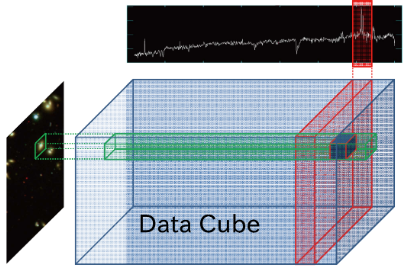
\includegraphics[width=0.45 \textwidth]{images/cube}
		\caption{The schematic illustration of a data cube of ALMA, with two spatial dimensions and a frequency or wavelength one \citep{eguchi_superluminal_2013}.}
		\label{fig:data_cube}
	\end{center}
\end{figure}